\documentclass{article}
\usepackage{amsfonts, amsmath, amssymb, amsthm} % Math notations imported
\usepackage{enumitem}
\usepackage{graphicx}
\usepackage[margin=1in]{geometry}
\graphicspath{ {.} }

\newtheorem{thm}{Theorem}
\newtheorem{prop}[thm]{Proposition}
\newtheorem{cor}[thm]{Corollary}

% title information
\title{Math 180A HW1}
\author{Neo Lee}
\date{01/18/2023}

% main content
\begin{document} 

% placing title information; comment out if using fancyhdr
\maketitle 

\textbf{Problem 3.}
\begin{enumerate}[label={(\alph*)}]
    \item 
    $\Omega = \{(1, 2, 3, 4, 5), (1, 2, 3, 4, 6), (1, 2, 3, 4, 7)\dots\}$ with no repetition of numbers in each element and orders do not matter, which means (1, 2, 3, 4, 5) is the same as (5, 4, 3, 2, 1). 
    There are a total of ${39 \choose 5} = 575757$ elements in $\Omega$. 
    \smallbreak
    Since each number are picked randomly and uniformly, the distribution of each element is uniform with $P = \frac{1}{|\Omega|} = \frac{1}{{39 \choose 5}}$.

    \item
    $P = \frac{{5 \choose 3} \times {(39 - 5) \choose 2}}{{39 \choose 5}} = \frac{10 \times 561}{575757} = \frac{5610}{575757}$ 
    \smallbreak
    We first choose 3 numbers out of the 5 numbers we have in our ticket. Then we choose 2 numbers out of the $(39 - 5) = 34$ numbers that are not on our ticket.
\end{enumerate}
\bigbreak

\textbf{Problem 4.}
\begin{enumerate}[label={(\alph*)}]
    \item 
    $\Omega = \{1C, 2C, 3C, \dots ,1D, 2D, \dots, 1H, 2H, \dots, 1S, 2S, \dots, 13S \}$ with C, D, H, S representing club, diamond, heart, and spade respectively.
    Therefore, there are a total of 52 elements in $\Omega$. 
    \smallbreak
    Since one card is picked randomly and uniformly, the probability measure is uniform for each event with $P = \frac{1}{|\Omega|} = \frac{1}{52}$.

    \item 
    We can define event $A$ as $(1S \cup 2S \cup 3S)$. \\
    Since $1S, 2S, 3S$ are disjoint, $P(A) = P(1S \cup 2S \cup 3S) = P(1S) + P(2S) + P(3S) = \frac{1}{52} + \frac{1}{52} + \frac{1}{52} = \frac{3}{52}$.
\end{enumerate}
\pagebreak
    
\textbf{Problem 5.}
\begin{enumerate}[label={(\alph*)}]
    \item 
    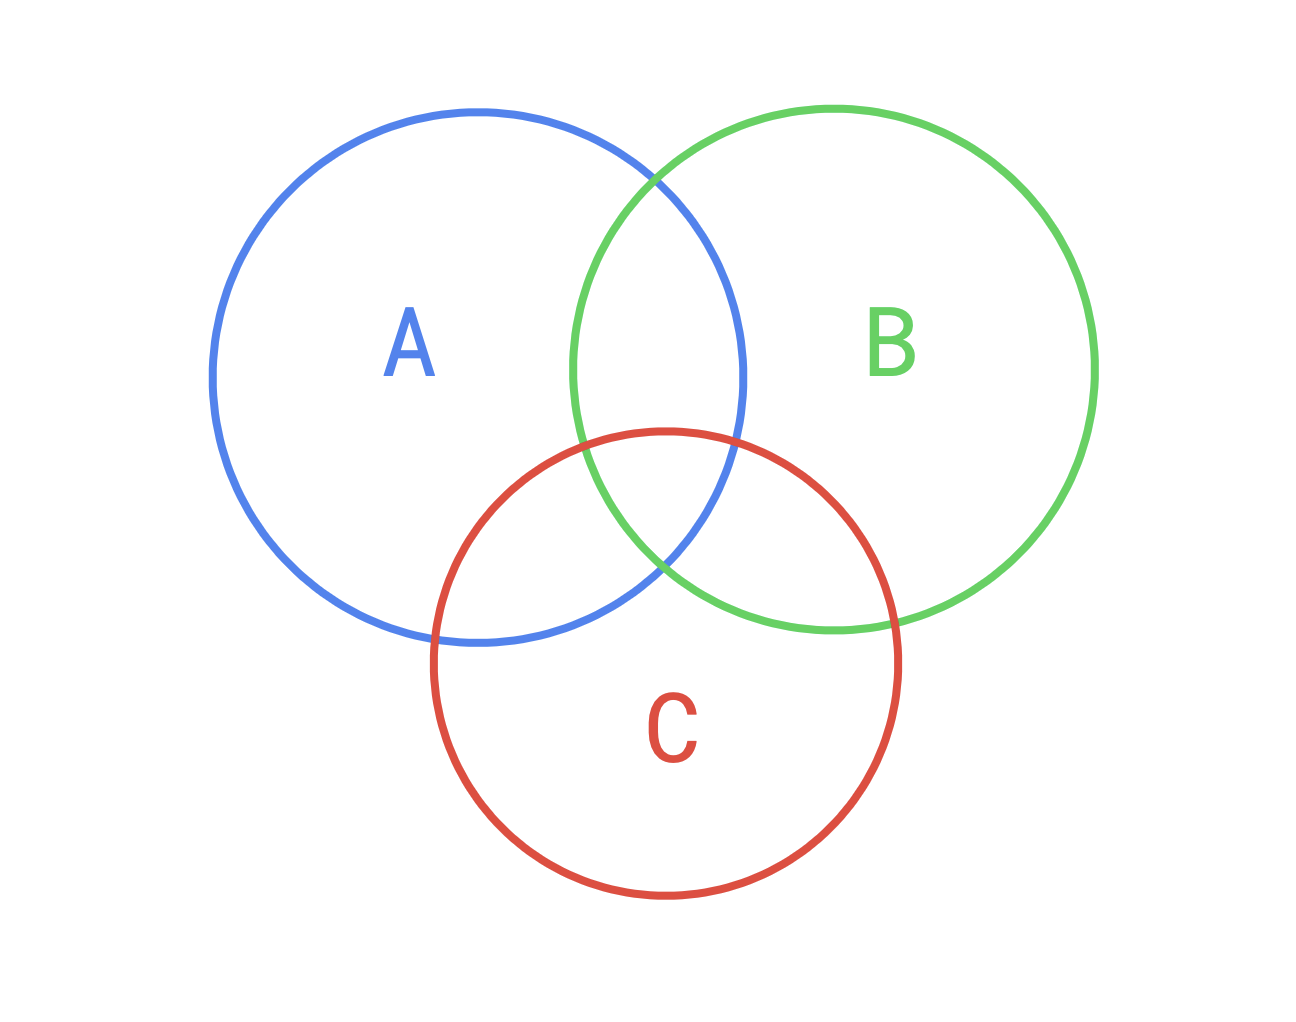
\includegraphics[width=0.5\textwidth]{venn_diagram}

    \item 
    $P(A \cup B \cup C) = P(A) + P(B) + P(C) - P(A \cap B) - P(A \cap C) - P(B \cap C) + P(A \cap B \cap C)$
    \smallbreak
    Let $p_1 = P(A \cap B^c \cap C^c), p_2 = P(A^c \cap B \cap C^c), p_3 = P(A^c \cap B^c \cap C), p_{12} = P(A \cap B \cap C^c), p_{13} = P(A \cap B^c \cap C), p_{23} = P(A^c \cap B \cap C), p_{123} = P(A \cap B \cap C)$. Note that all sets are pairwise disjoint.
    \smallbreak
    $P(A) + P(B) + P(C) - P(A \cap B) - P(A \cap C) - P(B \cap C) + P(A \cap B \cap C) \\
    = (p_1 + p_{12} + p_{13} + p_{123}) + (p_2 + p_{12} + p_{23} + p_{123}) + (p_3 + p_{13} + p_{23} + p_{123}) \\
    \indent - (p_{12} + p_{123}) - (p_{13} + p_{123}) - (p_{23} + p_{123}) + p_{123} \\
    = p_1 + p_2 + p_3 + p_{12} + p_{13} + p_{23} + p_{123} \\
    = P(A_1 \cup A_2 \cup A_3)$
\end{enumerate}
\bigbreak

\textbf{Problem 6.}
\begin{align}
    1 & \ge P(A \cup B) \\
    1 & \ge P(A) + P(B) - P(AB) \\
    1 & \ge 0.4 + 0.7 - P(AB) \\ 
    - 0.1 & \ge - P(AB) \\
    0.1 & \le P(AB)
\end{align}

We have proved that $0.1 \le P(AB)$.
\smallbreak
Since $(A \cap B) \subseteq A$ and $(A \cap B) \subseteq B$, $P(A \cap B) \le P(A)$ and $P(A \cap B) \le P(B)$. Therefore, $P(A \cap B) \le 0.4$. 
\smallbreak
In conclusion, $0.1 \le P(AB) \le 0.4$.
\pagebreak

\textbf{Problem 7.}
Let G = \{exactly two balls are green\}, R = \{exactly two balls are red\}, Y = \{exactly two balls are yellow\}, W = \{exactly two balls are white\}.
\begin{align}
    P(G \cup R \cup Y \cup W) = & P(G) + P(R) + P(Y) + P(W) \\
    & - P (G \cup R) - P(G \cup Y) -\dots \\
    & + P(G \cup R \cup Y) + P(G \cup R \cup W) + \dots \\
    & - P(G \cup R \cup Y \cup W)
\end{align}
Now let's calculate the individual terms:

\begin{align}
    P(G) = P(R) = \dots = \frac{{4 \choose 2} \times 3 \times 3}{4^4} = \frac{54}{256} = \frac{27}{128}\\
    P(G \cup R) = P(G \cup Y) = \dots = \frac{{4 \choose 2}}{4^4} = \frac{3 }{128}
\end{align}
Note that it's impossible for more than two of the events happen in the same time, therefore:
\begin{align}
    P(G \cup R \cup Y) = P(G \cup R \cup W) = \dots = P(G \cup R \cup Y \cup W) = 0
\end{align}
Therefore,
\begin{align}
    P(G \cup R \cup Y \cup W) & = 4 \times \frac{27}{128} - {4 \choose 2} \times \frac{3}{128} \\
    & = \frac{45}{64}
\end{align}
\bigbreak

\textbf{Problem 8.} \\
By inclusion-exclusion,
\begin{align}
    P(A_1 \cup A_2) = P(A_1) + P(A_2) - P(A_1 \cap A_2).
\end{align}
Since $P(A_1 \cap A_2) \ge 0$,
\begin{align}
    P(A_1 \cup A_2) \le P(A_1) + P(A_2).
\end{align}
Therefore, $P(A_1 \cup \dots \cup A_k) \le P(A_1) + \dots + P(A_k)$ is true for $k = 2$. \\
Suppose $P(A_1 \cup \dots \cup A_k) \le P(A_1) + \dots + P(A_k)$ is true for some natural numbers $k \ge 2$.
We get:
\begin{align}
    P(A_1 \cup \dots \cup A_k \cup A_{k+1}) = P(A_1 \cup \dots \cup A_k) + P(A_{k+1}) - P((A_1 \cup \dots \cup A_k) \cap A_{k+1}) 
\end{align}
Since $P((A_1 \cup \dots \cup A_k) \cap A_{k+1}) \ge 0$, 
\begin{align}
    P(A_1 \cup \dots \cup A_k \cup A_{k+1}) \le P(A_1 \cup \dots \cup A_k) + P(A_{k+1})
\end{align}
Since $P(A_1 \cup \dots \cup A_k) \le P(A_1) + \dots + P(A_k)$,
\begin{align}
    P(A_1 \cup \dots \cup A_k) + P(A_{k+1}) \le P(A_1) + \dots + P(A_k) + P(A_{k+1})
\end{align}
and 
\begin{align}
    P(A_1 \cup \dots \cup A_k \cup A_{k+1}) \le P(A_1) + \dots + P(A_k) + P(A_{k+1}).
\end{align}
Thus, $P(A_1 \cup \dots \cup A_k \cup A_{k+1}) \le P(A_1) + \dots + P(A_k) + P(A_{k+1})$ if the Induction Hypothesis is true. \\
Therefore, by Mathematical Induction, $P(A_1 \cup \dots \cup A_n) \le P(A_1) + \dots + P(A_n) = \sum_{k=1}^{n}P(A_k)$.

\end{document}